\subsection{Overview}
DDFEM is a combination of embedded finite elements and hierarchical
coarsening.
In this section, we discuss the problem of coarsening
and introduce the notion of a material palette. We conclude by
summarizing the two main stages of DDFEM—offline metamaterial
construction and online coarsening.
\paragraph{Coarsening for finite elements}
The key component of our DDFEM is coarsening.
Coarsening reduces the number of vertices in a finite element simulation mesh in order to improve
runtime performance.
Since simply removing vertices can greatly reduce
the accuracy of the simulation, coarsening schemes also assign
new materials to coarsened elements to minimize this effect.
We regard the global coarsening of a simulation mesh as the result
of many local coarsening operations which map from contiguous
subsets of fine elements with applied materials to coarse elements
with new, optimized materials. Our goal is to precompute these
optimized materials so that coarsening is fast at runtime. Below we
discuss how to make such a precomputation tractable beginning with
our choice of Finite Element simulation methodology.
\paragraph{Conforming vs. embedded finite elements}
The defining feature of conforming finite element methods is that the simulation
mesh is aligned with the geometry of the object being simulated.
One obvious feature of conforming meshes is that the mesh itself is a
function of the input geometry.
This means that the output of a local coarsening operator (the coarsened mesh) will also be a function
of the input geometry.
Also, the new material computed by each local coarsening operator will be a function of input geometry.
This dependence on input geometry is a significant issue to overcome
if we wish to precompute coarsened materials because, in design
problems, the input geometry is in constant flux.
The number of precomputed coarse materials now depends on the local material
assignment on the simulation mesh and the input geometry.
Thus space of coarsened materials is prohibitively large.
To mitigate this we turn to embedded finite elements.
These methods embed the geometry to be simulated into the simulation mesh with no regard
for whether the mesh conforms to the geometry or not.
Thus an identical simulation mesh can be used for any input geometry.
Local coarsening operations on the embedded mesh yield identical coarse
elements and the optimized coarse material depends only on the
local material distribution on the simulation mesh. This significantly
reduces the size of the coarsened material space. In this paper we
embed all simulation geometry into a hexahedral simulation mesh.
\paragraph{Material palette} We further shrink the space of coarsening operators
using an observation about material design. Designers do
not work in a continuous space of materials but limit themselves to
a relatively compact set (e.g. rubber, wood, steel) related to their
problem domain. We call these discrete sets of materials
palettes and denote them $\mathcal{P}=\{\mathcal{M}^1,...,\mathcal{M}^n\}$.
Here $\mathcal{M}^i$ denotes a specific material model in $\mathcal{P}$, 
and $n$ is the size of the material palette.
In this work we limit ourselves to nonlinear hyper-elastic materials,
which means that each $\mathcal{M}^i$ can be represented by a strain
energy density function.
We also include a void (or empty) material in every palette.
This allows us to perform topology changes in the
same manner in which we perform material assignment updates.
\paragraph{Algorithms}
With the material palette in hand, we can now define our algorithm, which is divided into two distinct phases: an \textbf{offline database construction} stage and an \textbf{online coarsening} stage.  Below we detail the input, output, and steps of each stage:
\vspace{1mm}
\hrule
\textbf{Offline Database Construction}
\vspace{1mm}
\hrule
\begin{compactitem}
	\item \textbf{INPUT:} A palette of materials to be applied to high-resolution hexahedral simulation meshes $\set{P}^0$
	\item \textbf{OUTPUT:} A new palette of coarse metamaterials, $\set{P}^1$, and a mapping from fine material combinations to the coarsened materials in $\set{P}^1$. 
	\item \textbf{STEPS:}
	\item \textbf{FOR EACH} material combination applied to a 2$\times$2$\times$2 cube of high resolution elements
	\subitem $\bullet$ Sample potential energy function of 2$\times$2$\times$2 block
	\subitem $\bullet$ Fit metamaterial for coarse hexahedral element
	\subitem $\bullet$ Add metamaterial to $\set{P}^1$ using high resolution 
	\subitem material IDs as database key
	\item \textbf{END}
\end{compactitem}
\vspace{1mm}
\hrule
\vspace{1mm}
\hrule
\textbf{Online Coarsening}
\vspace{1mm}
\hrule
\begin{compactitem}
	\item \textbf{INPUT:} High resolution hexahedral simulation mesh with 
	\subitem material IDs and
	\subitem coarsened hexahedral simulation mesh 
	\item \textbf{OUTPUT:} Metamaterial assignments for coarse mesh
	\item \textbf{STEPS:}
	\item \textbf{FOR EACH} 2$\times$2$\times$2 block in the high resolution mesh
	\subitem $\bullet$ Replace with single coarse element
	\subitem $\bullet$ Assign material from $\set{P}^1$ using high resolution 
	\subitem material IDs as database key 
	\item \textbf{END}
\end{compactitem}
\vspace{1mm}
\hrule

\paragraph{Hierarchical coarsening}
We stress that both stages of the DDFEM algorithm can be applied hierarchically. Given the first level of metamaterials, $\set{P}^1$, we can construct a metamaterial library, $\set{P}^2$, for the second level by using $\set{P}^1$ as an input material palette. At runtime, the coarsening algorithm looks up materials from $\set{P}^2$ to replace each 2$\times$2$\times$2 coarse block with a single element.

Having introduced the broad strokes of the DDFEM scheme, we move on to a detailed explanation of each algorithmic component. First we discuss database construction, followed by the runtime component. We end by demonstrating the speed and accuracy of DDFEM.
\subsection{title}
\section{Metamaterial Database Construction}
\label{sec:database}
We construct our metamaterial database using a potential energy fitting approach. This is valid due to the hyperelastic materials that make up our material palettes. Material fitting considers 2$\times$2$\times$2 blocks of high-resolution hexahedral elements (denoted $^0\set{E}$). For each element $^0E_k\in \, ^0\set{E}$, its material is referred to as $^0\set{M}_k\in \, ^0\set{P}$. (Note that $\set{E}$ refers to a set of elements and $E$ refers to a single element.) Given $^0\set{E}$, we can sample its deformation space, and using $^0\set{M}_k$, compute the potential energy $^0V$ for each sample.  Now we must find a metamaterial that, when applied to a single coarse element $^1\mathit{E}$ best approximates $^0V$.  This is accomplished by fitting a metamaterial potential energy function , $^1V$, to the set of deformation/energy samples. The fitted metamaterial is stored in the metamaterial database and indexed by the material indices of $^0\set{M}$.

\subsection{Metamaterial Model}
Our fitting approach depends on choosing a good metamaterial model.
In order to ensure that our model meets the criteria for a material energy function~\cite{Marsden2012}, we choose our metamaterial model for $^1\mathit{E}$ as a combination of material models of $^0\set{M}_k$:
\begin{align}
^1V(^1\vr{u}, \, ^1\vr{p}) = \sum_{k=1}^8 w_k \, ^0V_k(^0\vr{u}_k, \, ^1\vr{p}_k, \, ^1\vr{X}_k),
\label{eq:materialModel}
\end{align}
where $^0V_k$ is the strain energy density of $^0\set{M}_k$ at quadrature point position $^1\vr{X}_k$ (\autoref{fig:coarseFine}). Here $^1\vr{u}$ is the vector of nodal displacements associated with $^1\mathit{E}$ while $^0\vr{u}_k$ are displacements for the $k^{th}$ element at level $0$ reconstructed using trilinear interpolation from $^1\vr{u}$. The vector $^1\vr{p}$ stores the material parameters for the coarse metamaterial and consists of the stacked material parameter vectors for each material in $^0\set{M}_k$, themselves denoted by $^1\vr{p}_k$.  $w_k$ is the standard Gaussian quadrature weight.
We note that our model incurs slight computational overhead at runtime because we must evaluate potential energy functions at 8 quadrature points.
%However, because each constituent material model can be evaluated independently, much of this deficit can be made up by parallelizing the computation.
%Furthermore
However, the speed improvement gained by coarsening makes the remaining, per-quadrature point expense negligible.

\begin{figure}
	\centering
	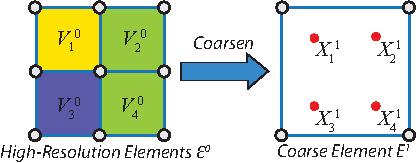
\includegraphics[width=0.6\textwidth]{images/coarseFine.pdf}
	\caption{The relationship between high-resolution and coarsened elements. At each quadrature point $^1\vr{X}_k$, the coarse element copies the corresponding energy density function $^0V_k$ from the high-resolution element.}
	\label{fig:coarseFine}
\end{figure}

We observe that even if the individual base material models are isotropic, the metamaterial can become anisotropic by assigning different material parameters at the quadrature points. We counter this by augmenting the metamaterial model with an anisotropic term, which improves fitting.
The complete model is then given by
\begin{align}
\begin{split}
^1V(^1\vr{u}, \, ^1\vr{p}, \, C) &= \sum_{k=1}^8 \bigg( w_k \, ^0V_k(^0\vr{u}, \, ^1\vr{p}_k, \, ^1\vr{X}_k)\\
& + C_k\left( \sqrt{\vr{v}^T\vr{F}_k^T\vr{F}_k\vr{v}} - 1\right)^2\bigg),\\
\label{eq:materialModel2}
\end{split}
\end{align}
where $\vr{v}$ is a unit-length direction of anisotropy and $C_k$ is the scaling parameter at the $k^{th}$ quadrature point. 

\subsection{Force Space Sampling}
\label{sec:force_space_sampling}
As mentioned previously, we take a sampling-based approach to metamaterial fitting. In order to fit our model (\autoref{eq:materialModel2}) to $^0V$ we first draw a number of samples from the deformation space of $^0\set{E}$ and compute $^0V$ for each sample.
If a user has prior knowledge of the set of meshes and simulations that they will require, then the best way to draw the samples is to run a number of anticipated simulations with various material combinations.
In this paper, we provide a more general method to draw samples for a metamaterial.
Initially, we attempted sampling by applying a random deformation to the corners of $^1\mathit{E}$; however, this led to many infeasible samples for very stiff materials.
In order to alleviate this problem we perform sampling in the force space.

For each element $^0\mathit{E}\in \, ^0\set{E}$ we apply a set of randomly generated forces.
We solve an elastostatic problem to compute the deformation of $^0\set{E}$, using constraints to remove rigid motion. Recall that this is fast because $^0\set{E}$ consists of just 8 elements.
Each sample is then a tuple $\left\{^0\vr{u}, \, ^0V\right\}$ (\autoref{fig:sampling}) where $^0\vr{u}$ are the nodal displacements of $^0\set{E}$, and $^0V$ is the strain energy density value of this deformed configuration.
\begin{figure}
	\centering
	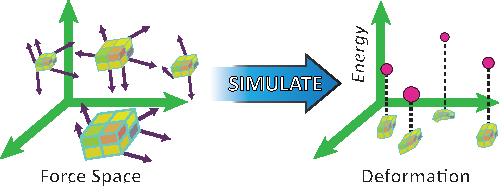
\includegraphics[width=0.8\columnwidth]{images/sampling.pdf}
	\caption{ We sample the energy function of a 2$\times$2$\times$2 block of hexahedra by applying random forces and deforming the block using FEM. Each set of forces results in a deformation-energy tuple which is used during fitting.}
	\label{fig:sampling}
\end{figure}

\subsection{Fitting}
\label{sec:fitting}
Given a set of deformation samples, $\left\{ ^0\vr{u}, \, ^0V\right\}$, we perform a least squares fit to determine the parameters, $^1\vr{p}$, for a given metamaterial (\autoref{fig:fitting}):
\begin{align}
^{1}\vr{p}^*= \underset{^1\vr{p}}{\operatorname{argmin}} \, \sum_{s=1}^{n_s}\left(^0V_s- \, ^1V\left(\vr{r}\left(^0\vr{u}_s\right), \, ^1\vr{p}\right)\right)^2,
\label{eq:fitting}
\end{align}
where $\vr{r}$ constructs $^1\vr{u}$ from $^0\vr{u}$, $n_s$ is the total number of samples, and $s$ indexes all samples. In our experiments we use the simplest form of $\vr{r}$ choosing it to extract the displacements of the corners of $^0\set{E}$.

\paragraph{Fitting in the Presence of Anisotropy}
If performed naively this optimization is nonlinear because we must simultaneously solve for $\vr{v}_k$, the preferred direction of anisotropy. This can severely slow the fitting procedure, especially in cases where it would otherwise be a linear least squares problem (i.e if all fine-scale materials are Neo-Hookean or a similarly simple material model).
To avoid this problem we first estimate all anisotropy directions, and then solve \autoref{eq:fitting} for the remaining material parameters.
Our intuition is that anisotropy manifests itself as preferential stretching along a particular axis. To find this axis, we apply stretching forces to a block in a discrete set of directions uniformly sampled over a sphere.
If the stretching force is close to the direction of anisotropy, then the amount of stretching deformation is reduced.
For any given stretching direction $\mathbf{v}$, we apply a stretching force and compute the deformation gradient $\mathbf{F}$ of  each quadrature point.
Under $\mathbf{F}$, a unit length vector in direction $\mathbf{v}$ is stretched to a new length $l = \|\mathbf{F}\mathbf{v}\|$.
The set of all 3D vectors $l\mathbf{v}$ forms an ellipse-like shape.
We find the principal axes of the ellipse (via SVD) and use them as directions of anisotropy.
\begin{figure}
	\centering
	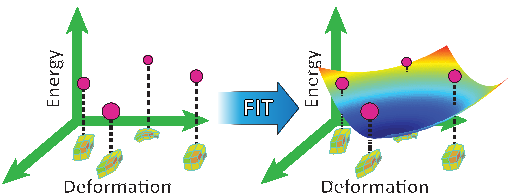
\includegraphics[width=0.8\columnwidth]{images/fitting.pdf}
	\caption{ Metamaterial potential energy functions are fitted to the deformation-energy samples using a least-squares optimization.}
	\label{fig:fitting}
\end{figure}
\paragraph{Regularization} Since vastly different material assignments, $^0\set{M}_k$, can produce the same metamaterial, our na\"{i}ve cost function (\autoref{eq:fitting}) can produce very large parameter values and even non-physical negative ones.
For example, consider a homogeneous material assignment at the high-resolution level.
The same metamaterial can be achieved by interleaving hard and soft materials at each fine element or by assigning a single, well chosen material to all fine elements.
To overcome this, we add a regularization term to control the parameter ranges and prevent overfitting of the training samples.
Our modified error function takes the following form:
\begin{equation}
\sum_{s=1}^{n_s}\left(^0V_s- \, ^1V\left(\vr{r}\left(^0\vr{u}_s\right), \, ^1\vr{p}\right)\right)^2 + 
\lambda\sum_k (^1\vr{p}_k - \, ^0\vr{p}_k)^2,
\end{equation}
which prevents material parameters from deviating too far from  $^0\set{M}_k$.
We chose the regularization constant $\lambda=0.02$ for the results in this paper.
In our experiments, since the base energy functions are linear with respect to the material parameters, the fitting problem can be solved by linear regression with regularization.

\begin{figure}
	\centering
	\includegraphics[width=0.8\columnwidth]{images/compression}
	\caption{Database compression step adds metamaterials to a compressed database by a farthest point sampling strategy.}
	\label{fig:compression}
\end{figure}

\subsection{Database Compression}
\label{sec:compression}
Given $n$ materials in the palette, the number of material combinations in a 2$\times$2$\times$2 block is $n^8$. In modern hardware, it is impossible to compute and store all material combinations even for a moderately-sized palette with $100$ materials.
In order to compress the number of materials stored in our metamaterial database, we select a small number of representative material combinations and remove all others. We compare materials in a feature space. In order to construct metamaterial feature vectors, we first select a common subset of deformations from all computed deformation samples. We then evaluate the potential energies of each metamaterial at each deformation sample. The stacked vector of energies becomes a metamaterial feature vector. 

Since our base materials differ in stiffness by orders of magnitude, we take the logarithm to measure the difference in ratio.
Let $D$ be the $L^2$ norm of log-energies between the two materials given by
\begin{equation}
D(A,B)=\sqrt{\sum_s (\log(^0V^{A}_{s})-\log(^0V^{B}_{s}))^2},
\end{equation} where $A$ and $B$ denote two distinct metamaterials in the database. 
Given the distance metric, we can select $k$ representatives materials using farthest point sampling~\cite{eldar1997farthest}. We randomly choose an initial metamaterial and then repeatedly select the material combination furthest away from any previous representatives -- continuing until we obtain $k$ representatives (\autoref{fig:compression}). This compression algorithm chooses $k$ samples that equally cover the metamaterial energy space, helping to preserve good behavior in our coarse simulations. 
\subsection{Hierarchical Coarsening}
While one level of coarsening can yield significant speed-ups, DDFEM can also be applied hierarchically.
As discussed in~\autoref{sec:compression}, the exponential growth of metamaterials palettes at each level makes it prohibitively expensive to perform fitting.
We address this by changing our coarsening strategy. 
Instead of choosing $^0\set{E}$ to be a 2$\times$2$\times$2 block we choose it to be a 2$\times$1$\times$1 block, which we coarsen. We construct an intermediate database of materials and compress. 
We then choose $^0\set{E}$ to be a 1$\times$2$\times$1 block, coarsen and compress, and finally a 1$\times$1$\times$2 block, coarsen and compress. Intermediate compression greatly reduces the number of samples we need to generate in order to populate the material parameter database for the next coarsening level. 
It is important to note that our intermediate databases only store lookup tables which allow us to extract appropriate material IDs for the next coarsening stage. Material parameters need only be stored in the final database since it is these elements that are simulated.
\begin{figure}
	\centering
	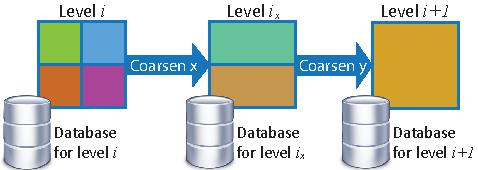
\includegraphics[width=0.7\textwidth]{images/hierchical}
	\caption{Hierarchical coarsening operates on one dimension at a time, performing clustering at each intermediate stage (here denoted $i_x$). This allows our compression algorithm to be applied aggressively, greatly reducing the number of energy samples we need for fitting material parameters. }
	\label{fig:hierarchy}
\end{figure}
\section{Runtime Simulation}
\label{sec:runtime}
Once our metamaterial database, $\set{P}^1$, has been constructed we can use it to perform fast online coarsening. 
Initially, the user loads geometry which is embedded in a hexahedral grid for simulation. Prior to simulation we iterate over all 2$\times$2$\times$2 blocks of hexahedral elements and perform mesh coarsening by replacing these 8 elements with a single coarse element. We perform a database lookup into $^1\set{P}$, using the material ID numbers of the 8 original elements, to quickly retrieve the optimal metamaterial for this coarse element. Database lookup is fast (even using our unoptimized, single-threaded implementation), and this is what makes DDFEM so appealing.
We achieve significant simulation speed-up from coarsening, retain accuracy in the simulation, and reduce the cost of material coarsening at runtime to a negligible amount.
	Our material model can be used in any simulation algorithm suitable for non-linear elasticity. In our experiments, we use Coin-IpOpt~\cite{ipopt} to implement static and dynamics simulations with tolerance (``tol'' option) set to $0.5$. We use Pardiso as our linear solver.
	For timing purposes, we limit Pardiso to single thread mode.
	The pseudo-code for static simulation is shown in \autoref{alg:sim}.
\begin{algorithm}[!h]
	
	\caption{Static Simulation}\label{alg:sim}
	\begin{algorithmic}[1]
		\REPEAT
		\STATE $\mathbf{f}$: global force vector
		\STATE $L$: triplet list for global stiffness matrix
		\FOR{each element e}
		\STATE compute elastic force $\mathbf{f}_e$
		\STATE add $\mathbf{f}_e$ to $\mathbf{f}$
		\ENDFOR
		\STATE add external force $\mathbf{f}_{ext}$ to $\mathbf{f}$
		\FOR{each element e}
		\STATE $\mathbf{K}_e$: element stiffness matrix
		\FOR{each quadrature point q}
		\STATE compute stiffness matrix $\mathbf{K}_q$ at quadrature point
		\STATE $\mathbf{K}_e+=\mathbf{K}_q$
		\ENDFOR
		\STATE append entries of $\mathbf{K}_e$ to $L$
		\ENDFOR
		\STATE sort $L$ to get sparse stiffness matrix $\mathbf{K}$
		\STATE set entries in $\mathbf{K}$ and $\mathbf{f}$ for fixed vertices
		\STATE $\Delta\mathbf{x}=\mathbf{K}^{-1}\mathbf{f}$
		\STATE compute step size $h$ using line-search
		\STATE $\mathbf{x}+=h\Delta\mathbf{x}$
		\UNTIL{convergence}
	\end{algorithmic}
\end{algorithm}